\documentclass[12pt]{article}
\usepackage{graphicx}
\usepackage{amssymb}

\begin{document}
%- https://www.tutorialspoint.com/discrete_mathematics/discrete_mathematics_sets.htm
\section*{Set Theory}

\newpage
German mathematician G. Cantor introduced the concept of sets. He had defined a set as a collection of definite and distinguishable objects selected by the means of certain rules or description.

Set theory forms the basis of several other fields of study like counting theory, relations, graph theory and finite state machines. In this chapter, we will cover the different aspects of Set Theory.


\subsection{Representation of a Set}
Sets can be represented in two ways −

Roster or Tabular Form
Set Builder Notation


%=====================================================%
\subsubsection*{Example 2} − The set ${1,3,5,7,9}$ is written as −

B={x:1\leqx<10 and (x%2)≠0}

If an element x is a member of any set S, it is denoted by x∈Sx∈S and if an element y is not a member of set S, it is denoted by y∉Sy∉S.

Example − If S={1,1.2,1.7,2},1∈SS={1,1.2,1.7,2},1∈S but 1.5∉S

Venn Diagrams
Venn diagram, invented in 1880 by John Venn, is a schematic diagram that shows all possible logical relations between different mathematical sets.

Examples

Venn Diagram



\subsection*{Subsets}

\begin{itemize}
\item Proper Subsets
\end{itemize}
\subsection*{The Power Set}

\newpage
\subsection*{Venn Diagrams}
\begin{figure}
\centering
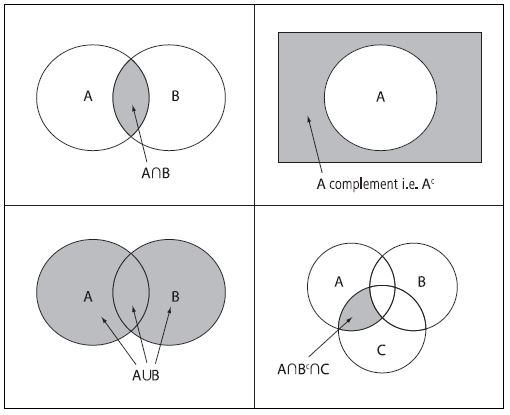
\includegraphics[width=0.7\linewidth]{venndiagram}

\end{figure}

\end{document}


